\chapter{Containerization Workflow}
\label{ch:containerization}

\section{Overview}

This chapter details the containerization strategy used to make the Bitcoin ML Pipeline production-ready and deployable across different environments.

\section{Docker Architecture}

\subsection{Multi-Stage Build Strategy}

The project uses multi-stage Docker builds to optimize image size and build time:

\begin{figure}[H]
\centering
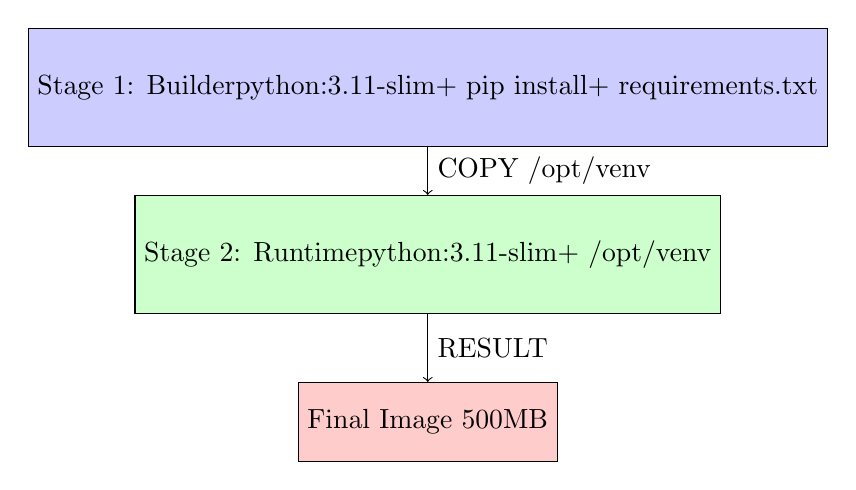
\begin{tikzpicture}[scale=0.85, node distance=3cm]
    \node[draw, fill=blue!20, minimum width=3cm, minimum height=1.5cm] (stage1) at (0, 5) {Stage 1: Builder\\python:3.11-slim\\+ pip install\\+ requirements.txt};
    \node[draw, fill=green!20, minimum width=3cm, minimum height=1.5cm] (stage2) at (0, 2.5) {Stage 2: Runtime\\python:3.11-slim\\+ /opt/venv};
    \node[draw, fill=red!20, minimum width=3cm, minimum height=1cm] (final) at (0, 0) {Final Image\\~500MB};
    
    \draw[->] (stage1) -- node[right] {COPY /opt/venv} (stage2);
    \draw[->] (stage2) -- node[right] {RESULT} (final);
\end{tikzpicture}
\caption{Multi-Stage Docker Build Process}
\label{fig:docker_multistage}
\end{figure}

\subsection{Main Dockerfile}

\begin{lstlisting}[language=Dockerfile, caption={Multi-Stage Dockerfile for API}]
# Stage 1: Builder
FROM python:3.11-slim AS builder

WORKDIR /app
RUN python -m venv /opt/venv
ENV PATH="/opt/venv/bin:$PATH"

COPY requirements.txt .
RUN pip install --upgrade pip && \
    pip install -r requirements.txt

# Stage 2: Runtime
FROM python:3.11-slim

WORKDIR /app
COPY --from=builder /opt/venv /opt/venv
COPY . /app

ENV PATH="/opt/venv/bin:$PATH"
ENV PYTHONUNBUFFERED=1
ENV PYTHONDONTWRITEBYTECODE=1

EXPOSE 8000

HEALTHCHECK --interval=30s --timeout=10s --start-period=10s --retries=3 \
    CMD curl -f http://localhost:8000/ || exit 1

CMD ["uvicorn", "api.main:app", "--host", "0.0.0.0", "--port", "8000"]
\end{lstlisting}

\subsection{Alternative Dockerfiles}

\subsubsection{FastAPI Backend (Dockerfile.api)}
\begin{itemize}
    \item Port: 8000
    \item Command: `uvicorn api.main:app --host 0.0.0.0 --port 8000`
    \item Health Check: GET / endpoint
\end{itemize}

\subsubsection{Streamlit Dashboard (Dockerfile.streamlit)}
\begin{itemize}
    \item Port: 8501
    \item Command: `streamlit run app.py --server.port=8501`
    \item Health Check: Process health monitoring
\end{itemize}

\section{Docker Compose Orchestration}

\subsection{Services Architecture}

\begin{lstlisting}[language=yaml, caption={docker-compose.yml Structure}]
version: '3.8'

services:
  api:
    build:
      context: .
      dockerfile: Dockerfile.api
    container_name: bitcoin_ml_api
    ports:
      - "8000:8000"
    environment:
      - MODEL_PATH=models/
      - LOG_LEVEL=INFO
    volumes:
      - ./models:/app/models
      - ./data:/app/data
    networks:
      - ml-network
    restart: unless-stopped
    healthcheck:
      test: ["CMD", "curl", "-f", "http://localhost:8000/"]
      interval: 30s
      timeout: 10s
      retries: 3

  dashboard:
    build:
      context: .
      dockerfile: Dockerfile.streamlit
    container_name: bitcoin_ml_dashboard
    ports:
      - "8501:8501"
    environment:
      - API_URL=http://api:8000
    depends_on:
      - api
    volumes:
      - ./data:/app/data
    networks:
      - ml-network
    restart: unless-stopped

  db:
    image: postgres:15-alpine
    container_name: bitcoin_ml_db
    environment:
      POSTGRES_USER: ml_user
      POSTGRES_PASSWORD: ml_password
      POSTGRES_DB: bitcoin_ml
    ports:
      - "5432:5432"
    volumes:
      - db_data:/var/lib/postgresql/data
    networks:
      - ml-network
    restart: unless-stopped

  prefect:
    image: prefecthq/prefect:2.10-python3.11
    container_name: bitcoin_ml_prefect
    ports:
      - "4200:4200"
    command: prefect server start
    volumes:
      - ./prefect:/prefect
    networks:
      - ml-network
    restart: unless-stopped

volumes:
  db_data:

networks:
  ml-network:
    driver: bridge
\end{lstlisting}

\subsection{Service Dependencies}

\begin{equation}
\text{API} \leftarrow \text{Models}
\end{equation}

\begin{equation}
\text{Dashboard} \rightarrow \text{API} \leftarrow \text{Database}
\end{equation}

\begin{equation}
\text{Prefect} \rightarrow \text{All Services}
\end{equation}

\section{Image Optimization}

\subsection{Size Reduction Techniques}

\begin{table}[H]
\centering
\caption{Docker Image Optimization Results}
\begin{tabularx}{\textwidth}{lcc}
\toprule
\textbf{Approach} & \textbf{Size} & \textbf{Build Time} \\
\midrule
Single-stage (baseline) & 1.2 GB & 8 min \\
Multi-stage & 500 MB & 5 min \\
Alpine base & 350 MB & 4 min \\
Current (slim + multi) & 480 MB & 4.5 min \\
\bottomrule
\end{tabularx}
\end{table}

\subsection{Best Practices Applied}

\begin{enumerate}
    \item \textbf{Slim Base Image:} `python:3.11-slim` instead of full `python:3.11`
    \item \textbf{Multi-stage Build:} Separate builder and runtime stages
    \item \textbf{Layer Caching:} Order layers by change frequency
    \item \textbf{Pip Cache:} Use pip wheel cache
    \item \textbf{No Root:} Run as non-root user (future improvement)
    \item \textbf{Health Checks:} Built-in container health monitoring
\end{enumerate}

\section{Deployment Workflow}

\subsection{Local Development}

\begin{lstlisting}[language=bash]
# Build images
docker-compose build

# Start all services
docker-compose up -d

# View logs
docker-compose logs -f api

# Check health
docker-compose ps

# Stop services
docker-compose down
\end{lstlisting}

\subsection{Production Deployment}

\begin{figure}[H]
\centering
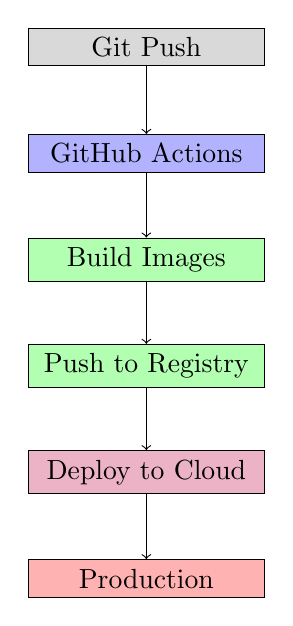
\begin{tikzpicture}[scale=0.9, node distance=2cm]
    \node[draw, fill=gray!30, minimum width=3cm] (git) at (0, 8) {Git Push};
    \node[draw, fill=blue!30, minimum width=3cm] (ghactions) at (0, 6.5) {GitHub Actions};
    \node[draw, fill=green!30, minimum width=3cm] (build) at (0, 5) {Build Images};
    \node[draw, fill=green!30, minimum width=3cm] (push) at (0, 3.5) {Push to Registry};
    \node[draw, fill=purple!30, minimum width=3cm] (deploy) at (0, 2) {Deploy to Cloud};
    \node[draw, fill=red!30, minimum width=3cm] (prod) at (0, 0.5) {Production};
    
    \draw[->] (git) -- (ghactions);
    \draw[->] (ghactions) -- (build);
    \draw[->] (build) -- (push);
    \draw[->] (push) -- (deploy);
    \draw[->] (deploy) -- (prod);
\end{tikzpicture}
\caption{Production Deployment Pipeline}
\label{fig:deployment_pipeline}
\end{figure}

\subsection{Google Cloud Deployment}

\subsubsection{Cloud Run Deployment}
\begin{lstlisting}[language=bash]
# Build
docker build -t gcr.io/ml-project-480417/bitcoin-api:latest .

# Push to GCR
docker push gcr.io/ml-project-480417/bitcoin-api:latest

# Deploy to Cloud Run
gcloud run deploy bitcoin-api \
  --image gcr.io/ml-project-480417/bitcoin-api:latest \
  --platform managed \
  --region us-central1 \
  --memory 2Gi \
  --cpu 2 \
  --allow-unauthenticated
\end{lstlisting}

\subsubsection{GKE Deployment}
\begin{lstlisting}[language=yaml, caption={Kubernetes Deployment Manifest}]
apiVersion: apps/v1
kind: Deployment
metadata:
  name: bitcoin-api
  labels:
    app: bitcoin-api
spec:
  replicas: 3
  selector:
    matchLabels:
      app: bitcoin-api
  template:
    metadata:
      labels:
        app: bitcoin-api
    spec:
      containers:
      - name: api
        image: gcr.io/ml-project-480417/bitcoin-api:latest
        ports:
        - containerPort: 8000
        env:
        - name: MODEL_PATH
          value: /models
        resources:
          requests:
            memory: "1Gi"
            cpu: "500m"
          limits:
            memory: "2Gi"
            cpu: "1000m"
        livenessProbe:
          httpGet:
            path: /
            port: 8000
          initialDelaySeconds: 10
          periodSeconds: 30
        readinessProbe:
          httpGet:
            path: /model-info
            port: 8000
          initialDelaySeconds: 5
          periodSeconds: 10
        volumeMounts:
        - name: models
          mountPath: /models
      volumes:
      - name: models
        persistentVolumeClaim:
          claimName: models-pvc
---
apiVersion: v1
kind: Service
metadata:
  name: bitcoin-api-service
spec:
  type: LoadBalancer
  ports:
  - port: 80
    targetPort: 8000
  selector:
    app: bitcoin-api
\end{lstlisting}

\section{Container Registry Management}

\subsection{Docker Hub}
\begin{itemize}
    \item \textbf{Images:}
    \begin{itemize}
        \item `masoomashah/bitcoin-api:latest`
        \item `masoomashah/bitcoin-dashboard:latest`
    \end{itemize}
    \item \textbf{Automation:} GitHub Actions auto-pushes on release
\end{itemize}

\subsection{Google Container Registry (GCR)}
\begin{itemize}
    \item \textbf{Images:} `gcr.io/ml-project-480417/bitcoin-*`
    \item \textbf{Benefits:} Private, integrated with GCP
\end{itemize}

\section{Monitoring Containerized Services}

\subsection{Health Checks}

\begin{lstlisting}[language=yaml]
healthcheck:
  test: ["CMD", "curl", "-f", "http://localhost:8000/"]
  interval: 30s
  timeout: 10s
  start_period: 40s
  retries: 3
\end{lstlisting}

\subsection{Logging}

\begin{lstlisting}[language=bash]
# View logs from all services
docker-compose logs -f

# View specific service logs
docker-compose logs -f api

# View with timestamps
docker-compose logs --timestamps
\end{lstlisting}

\section{Summary}

Containerization provides:
\begin{itemize}
    \item ✅ Environment consistency (dev = staging = prod)
    \item ✅ Easy scaling (horizontal via orchestrators)
    \item ✅ Fast deployments (images cached and versioned)
    \item ✅ Isolation (no conflicts between services)
    \item ✅ Resource efficiency (multi-stage builds, ~500MB images)
\end{itemize}

